\documentclass{beamer}
\usepackage{tikz,amsmath,amssymb,hyperref,graphicx,stackrel,setspace,animate,listings}
\usetikzlibrary{positioning,shadows,arrows,shapes,calc}
\newcommand{\argmax}{\operatornamewithlimits{argmax}}
\newcommand{\argmin}{\operatornamewithlimits{argmin}}
\mode<presentation>{\usetheme{Frankfurt}}
\DeclareMathOperator*{\softmax}{softmax}
\AtBeginSection[]
{
  \begin{frame}<beamer>
    \frametitle{Outline}
    \tableofcontents[currentsection,currentsubsection]
  \end{frame}
}
\title{Lecture 11: Adaboost and the Viola-Jones Face Detector}
\author{Mark Hasegawa-Johnson\\These slides are in the public domain}
\date{ECE 417: Multimedia Signal Processing, Fall 2023}  
\begin{document}

% Title
\begin{frame}
  \maketitle
\end{frame}

% Title
\begin{frame}
  \tableofcontents
\end{frame}


%%%%%%%%%%%%%%%%%%%%%%%%%%%%%%%%%%%%%%%%%%%%
\section[Review]{Review: Neural Network}
\setcounter{subsection}{1}

\begin{frame}
  \frametitle{Review: Images}

  An image is a signal, or a stack of signals.  Often we write
  $I[c,m,n]$ where $c$ is the color ($c\in\{1,2,3\}$), $m$ is the row
  index, and $n$ is the column index.
\end{frame}
  
\begin{frame}
  \frametitle{Review: Convolutional Neural Nets}
  \begin{enumerate}
  \item Forward-prop is convolution:
    \begin{align*}
      Z[d,m,n] &= W[d,c,m,n] \ast I[c,m,n]
    \end{align*}
  \item Back-prop is correlation:
    \begin{align*}
      \frac{\partial{\mathcal L}}{\partial I[c,m,n]} &=
      W[d,c,m,n] \bigstar \frac{\partial{\mathcal L}}{\partial Z[d,m,n]}
    \end{align*}
  \item Weight gradient is correlation:
    \begin{align*}
      \frac{\partial{\mathcal L}}{\partial W[d,c,m,n]} &=
      \frac{\partial{\mathcal L}}{\partial Z[d,m,n]} \bigstar I[c,m,n]
    \end{align*}
  \end{enumerate}
\end{frame}

%%%%%%%%%%%%%%%%%%%%%%%%%%%%%%%%%%%%%%%%%%%%
\section[Detection]{The Face Detection Problem}
\setcounter{subsection}{1}

\begin{frame}
  \centerline{\includegraphics[width=\textwidth]{exp/face_detection.jpg}}
  \url{https://commons.wikimedia.org/wiki/File:Face_detection.jpg}
\end{frame}

\begin{frame}[fragile]
  \frametitle{Face Detection: Problem Definition}

  \begin{lstlisting}
    for m in range(M):
      for n in range(N):
        for height in range(number_rows - row):
          for width in range(number_cols - col):
            does (m,n,height,width) contain a face?
\end{lstlisting}

\end{frame}

\begin{frame}
  \frametitle{Why is Face Detection Difficult?}

  A CNN face detector might detect a face of width $w$ and height $h$
  by training a ``face detector'' filter, $f[m,n]$ of width $w$
  and height $h$, then filtering the whole image to find the $(m,n)$
  where the face is located:
  \begin{align*}
    Z_{w,h}[m,n] &= f_{w,h}[m,n] \ast I[m,n]
  \end{align*}
  If the image is $M\times N$, this operation requires $w\times
  h\times M\times N$ multiplications.
\end{frame}
\begin{frame}
  \frametitle{Faces Come in Many Different Sizes}
  \centerline{\includegraphics[width=0.8\textwidth]{exp/fraunhofer.jpg}}
  \url{https://commons.wikimedia.org/wiki/File:Fraunhofer_-_Face_Detection_-_4406340595.jpg}
\end{frame}

\begin{frame}
  \frametitle{Faces Come in Many Different Sizes}
  \begin{itemize}
  \item Suppose the face width can be any size between $1\le w\le W$
  \item Suppose the face height can be any size between $1\le h\le H$
  \item Then we need $WH$ different filters, $f_{w,h}[m,n]$, so that
    we can detect all the different faces
  \item Total computational complexity is:
    \begin{displaymath}
      \sum_{w=1}^W\sum_{h=1}^H whMN = \frac{1}{4}(W+1)^2(H+1)^2MN~\text{multiplications/image}
    \end{displaymath}
  \end{itemize}
\end{frame}

%%%%%%%%%%%%%%%%%%%%%%%%%%%%%%%%%%%%%%%%%%%%
\section[Features]{Haar-Like Features}
\setcounter{subsection}{1}

\begin{frame}
  \frametitle{Haar-Like Features}

  Viola and Jones (2004) proposed solving the computational complexity
  problem by using very simple filters that they called ``Haar-like
  features,'' because they resemble Haar wavelets.
  \begin{enumerate}
  \item Haar-like features require no multiplications, because for all
    $n$, $f[n]$ is either $-1$ or $+1$.
  \item Haar-like features also require very few additions, because of
    a neat trick called the ``integral image.''
  \end{enumerate}
\end{frame}

\begin{frame}
  \frametitle{(1) Haar-like features require no multiplication}

  Haar-like features are convolutions, $Z[m,n]=f[m,n]\ast I[m,n]$, but
  the filters are $f[m,n]\in\{-1,1\}$.  Shown below are 2-rectangle,
  3-rectangle, and 4-rectangle filters.  The black pixels are
  $f[m,n]=+1$, the white pixels are $f[m,n]=-1$. 

  \centerline{\includegraphics[height=1in]{exp/haarlike.png}}
  \url{https://commons.wikimedia.org/wiki/File:VJ_featureTypes.svg}
\end{frame}

\begin{frame}
  \frametitle{(2) Haar-like features require few additions}

  Haar-like feature require very few additions, because they take
  advantage of an intermediate computation called the \textbf{integral
    image:}
  \begin{displaymath}
    II[m,n] = \sum_{m'=1}^m\sum_{n'=1}^n I[m',n'],~~~1\le m\le M,1\le n\le N
  \end{displaymath}
  The integral image is computed just once, for the entire image.
\end{frame}

\begin{frame}
  \frametitle{Summing a rectangle: Three additions}

  Using the integral image, the sum of all pixels inside a rectangle
  can be computed with only three additions.
  \begin{displaymath}
    \sum_{m'=m}^{m+h}\sum_{n'=n}^{n+w}I[m',n'] = II[m+h,n+w]-II[m,n+w]-II[m+h,n]+II[m,n]
  \end{displaymath}
  
  \centerline{\includegraphics[height=1.25in]{exp/rectangle.png}}
  \url{https://commons.wikimedia.org/wiki/File:Prm_VJ_fig3_computeRectangleWithAlpha.png}
\end{frame}



\begin{frame}
  \begin{columns}
    \begin{column}{0.5\textwidth}
      \begin{align*}
        &\sum_{m'=m}^{m+h}\sum_{n'=n}^{n+w}I[m',n']\\
        &= II[m+h,n+w]-II[m,n+w]\\
        &-II[m+h,n]+II[m,n]
      \end{align*}
      Figure: \url{https://commons.wikimedia.org/wiki/File:Integral_image_application_example.svg}
    \end{column}
    \begin{column}{0.5\textwidth}
      \centerline{\includegraphics[height=\textheight]{exp/integralimage.png}}
    \end{column}
  \end{columns}
\end{frame}

\begin{frame}
  \frametitle{The Training Token}

  Suppose we have a particular training datum $x$, which is an image
  from the training database, $I$, and a corresponding rectangle
  specifier $(r_1,r_2,r_3,r_4)=$(horizontal,vertical,width,height):
  \begin{displaymath}
    x=\left[\begin{array}{ccc}
        I[r_2,r_1]&\cdots&I_i[r_2,r_1+r_3]\\
        \vdots&\ddots&\vdots\\
        I_i[r_2+r_4,r_1]&\cdots&I_i[r_4+r_2,r_1+r_3]
      \end{array}\right]
  \end{displaymath}
  What are the different features we can compute from this image?
\end{frame}

\begin{frame}
  \frametitle{The Features}
  Viola \& Jones define Haar-like features specified by:
  \begin{itemize}
  \item $(\phi_i,\phi_2)$: Upper-left-corner of the sub-rectangle
    within the face rectangle, expressed as a fraction of the
    face rectangle, i.e., the upper left corner is
    $[m,n]=(r_2+r_4\phi_2,r_1+r_3\phi_1)$
  \item $(\phi_3,\phi_4)$: Size of the sub-rectangle, expressed as
    a fraction of the face rectangle size, i.e., width in pixels
    is $r_3\phi_3$, height in pixels is $r_4\phi_4$
  \item $(o_1,o_2)$: number of blocks in the horizontal and
    vertical directions, respectively.
  \end{itemize}
\end{frame}
\begin{frame}
  \frametitle{The Features}
  For example, here is a feature specified by $f=(\phi_1,\phi_2,\phi_3,\phi_4,o_1,o_2)=\left(\frac{1}{6},\frac{1}{6},\frac{2}{3},\frac{1}{3},2,1\right)$:
  \centerline{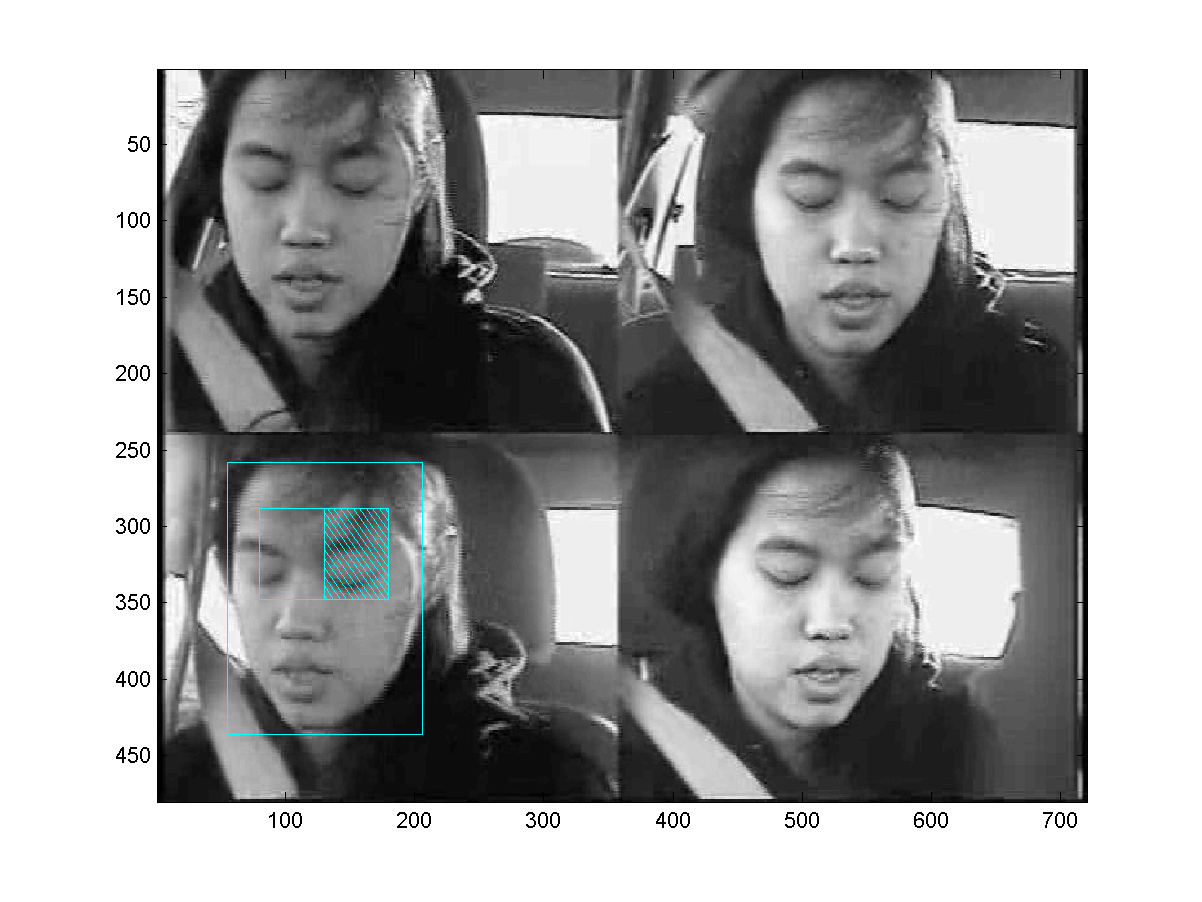
\includegraphics[height=0.7\textheight]{figs/2rectangle_feature.png}}
\end{frame}


%%%%%%%%%%%%%%%%%%%%%%%%%%%%%%%%%%%%%%%%%%%%
\section[Weak Classifier]{The Weak Classifier}
\setcounter{subsection}{1}

\begin{frame}
  \frametitle{The Weak Classifier}

  Viola \& Jones define the $j^{\text{th}}$ ``weak classifier'' in
  terms of a feature $f_j(\cdot)$, a sign $p_j\in\{-1,1\}$, and a
  threshold $\theta_j\in\Re$:
  \begin{displaymath}
    h_j(x)=\left\{\begin{array}{ll}
    1 & p_jf_j(x) < p_j\theta_j\\
    0 & \mbox{otherwise}
    \end{array}\right.
  \end{displaymath}
\end{frame}

\begin{frame}
  \frametitle{The Weak Classifier: Complete Specification}

  Putting it all together, a ``weak classifier,'' $f_j$, is specified
  by 8 numbers:
  \begin{itemize}
  \item $(\phi_{j,1},\phi_{j,2},\phi_{j,3},\phi_{j,4})$: position of the subrectangle
    within the candidate face rectangle
  \item $(o_{j,1},o_{j,2})$: number of blocks within the subrectangle
  \item $\theta_j$: threshold above or below which we should detect a face
  \item $p_j$: sign of the weak classifier: are faces detected by
    being below (+1) or above (-1) the threshold feature value?
  \end{itemize}
\end{frame}

\begin{frame}
  \frametitle{Selecting the Weak Classifier}

  \begin{itemize}
    \item 
      How do we choose $(\phi_{1},\phi_{2},\phi_{3},\phi_{4},o_1,o_2,p,\theta)$?
    \item
      To start with, let's suppose that we are evaluating a candidate
      feature,
      $f_j=(\phi_{j,1},\phi_{j,2},\phi_{j,3},\phi_{j,4},o_{j,1},o_{j,2})$.
    \item 
      We want to find the values of $p_j$ and $\theta_j$ that minimize
      the training corpus error rate for this $f_j$, and we want to
      calculate the value of that error rate.
  \end{itemize}
\end{frame}

\begin{frame}
  \frametitle{Feature Values, Weights, and Labels}
  \begin{columns}
    \begin{column}{0.4\textwidth}
      \begin{itemize}
      \item For every training token $x_i$, find the feature value
        $f_j(x_i)$.
      \item Second, assign a weight to every token, $w_j(x_i)$.  To
        start with, all the weights are equal, $w_j(x_i)=\frac{1}{n}$
        where $n$ is the number of tokens.
      \item Third, list the target labels, $y_i\in\{1,0\}$.
      \end{itemize}
    \end{column}
    \begin{column}{0.6\textwidth}
      \centerline{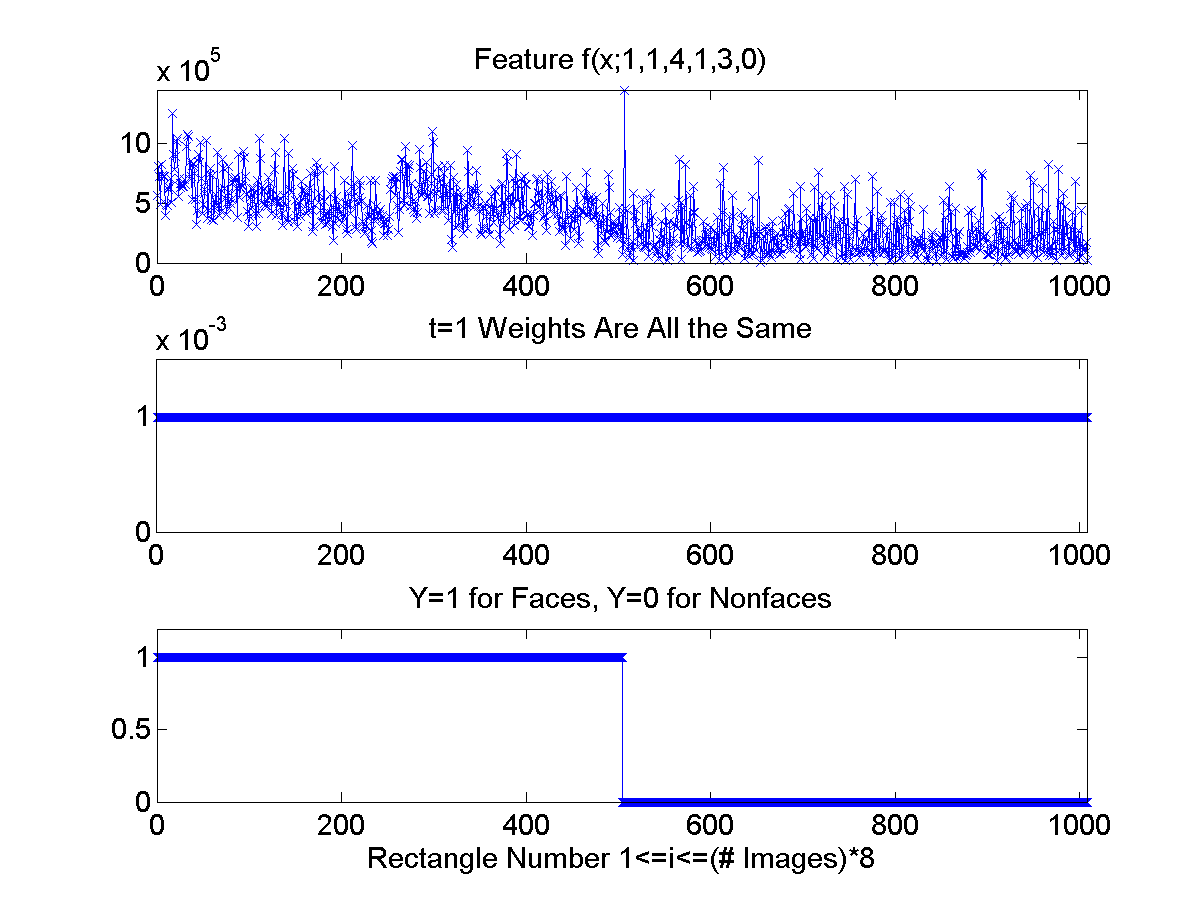
\includegraphics[width=\textwidth]{figs/features_weights_labels.png}}
    \end{column}
  \end{columns}
\end{frame}
      
\begin{frame}
  \frametitle{Feature Values, Weights$\times$ Labels}
  \begin{columns}
    \begin{column}{0.4\textwidth}
      \begin{itemize}
      \item Convert the labels from $\{0,1\}$ to $\{-1,1\}$
      \item Multiply each label times its weight, to give its ``signed importance:''
        \begin{displaymath}
          s_i = w(x_i)\times (2y_i-1)
        \end{displaymath}
      \end{itemize}
    \end{column}
    \begin{column}{0.6\textwidth}
      \centerline{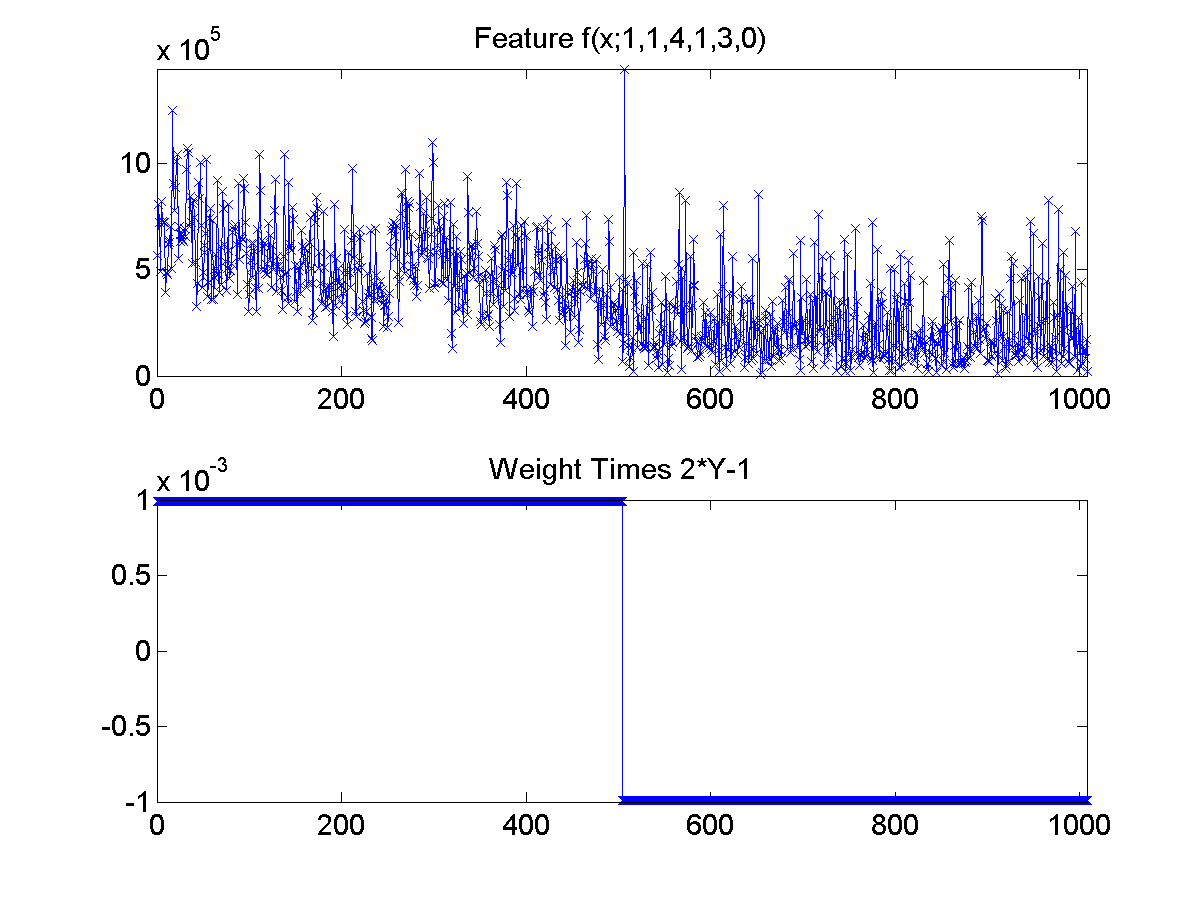
\includegraphics[width=\textwidth]{figs/features_weightslabels.png}}
    \end{column}
  \end{columns}
\end{frame}
      
\begin{frame}
  \frametitle{Sorted Features, Argsorted Weights$\times$ Labels}
  \begin{columns}
    \begin{column}{0.4\textwidth}
      \begin{itemize}
        \item 
          Now sort all the tokens in ascending order of their feature value.
        \item
          In the example here, you can see immediately that large
          feature values tend to be associated with the label $y_i=1$,
          and small feature values with $y_i=0$, though there's a lot
          of variability.
      \end{itemize}
    \end{column}
    \begin{column}{0.6\textwidth}
      \centerline{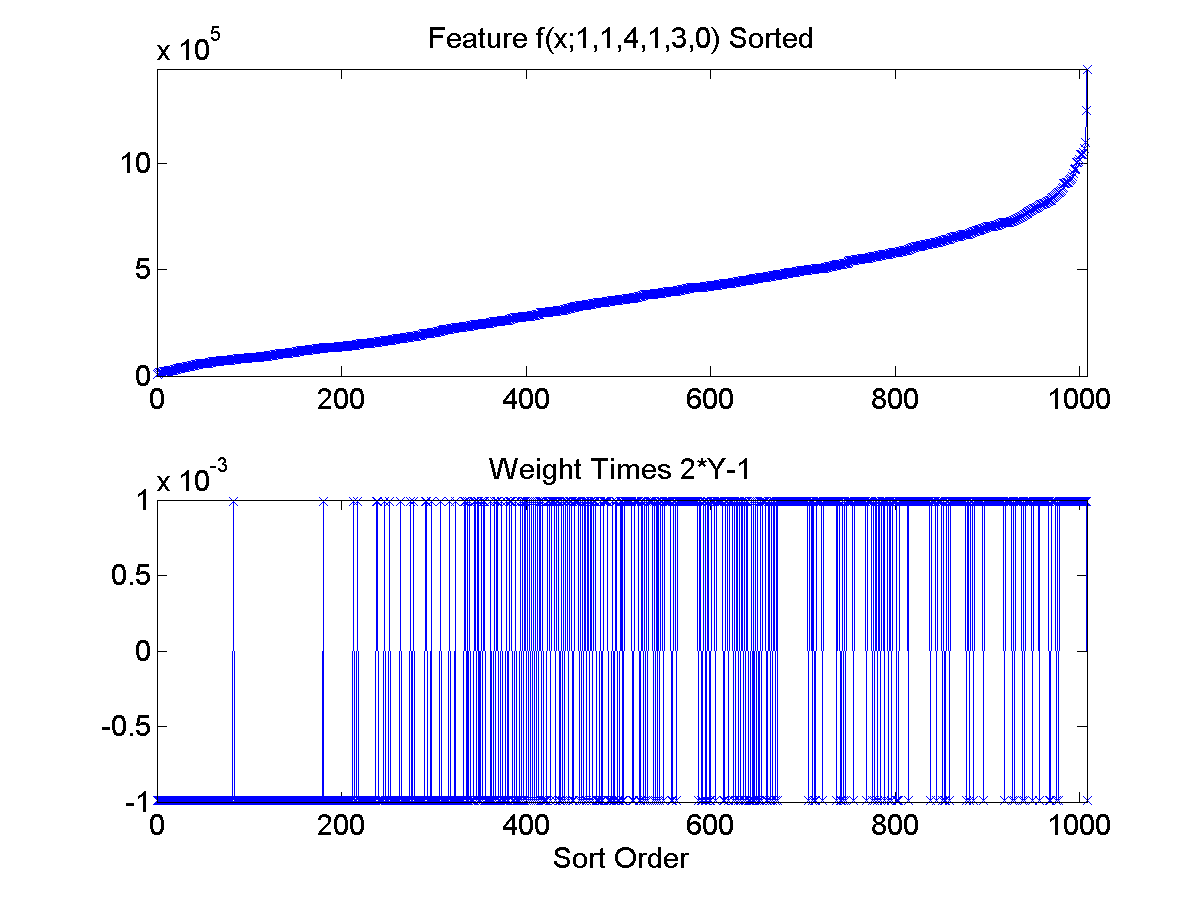
\includegraphics[width=\textwidth]{figs/features_weightslabels_sorted.png}}
    \end{column}
  \end{columns}
\end{frame}

\begin{frame}
  \frametitle{True Reject, False Reject, True Accept, False Accept}
  \begin{columns}
    \begin{column}{0.5\textwidth}
      \begin{itemize}
        \item 
          If $h_j(x_i)=0$, we say that the classifier ``rejects'' the token.
        \item
          If $h_j(x_i)=1$, we say the classifier ``accepts'' the token.
        \item
          If $h_j(x_i)=y_i$, we call this a ``true accept'' or ``true reject.''
        \item
          If $h_j(x_i)\ne y_i$, we call it a ``false accept'' or ``false reject.''
      \end{itemize}
    \end{column}
    \begin{column}{0.5\textwidth}
      \centerline{\begin{tabular}{c|cc|}
      &$f_j(x_i)=0$&$f_j(x_i)=1$\\\hline
      $y_i=0$ & TR & FA \\
      $y_i=1$ & FR & TA \\\hline
      \end{tabular}}
    \end{column}
  \end{columns}
\end{frame}

\begin{frame}
  \frametitle{True Reject, False Reject, True Accept, False Accept}

  \begin{itemize}
  \item If $p_j=+1$, the classifier {\bf accepts} any token with $f_j(x_i)<\theta_j$:
    \begin{align*}
      \Pr(FA|p_j=1) = \Pr(f_j(x_i)<\theta_j,y_i=0) &= \sum_{i:f_j(x_i)<\theta_j} w_j(x_i)(1-y_i)\\
      \Pr(TA|p_j=1) = \Pr(f_j(x_i)<\theta_j,y_i=1) &= \sum_{i:f_j(x_i)<\theta_j} w_j(x_i)y_i
    \end{align*}
  \item If $p_j=-1$, the classifier {\bf rejects} any token with $f_j(x_i)<\theta_j$:
    \begin{align*}
      \Pr(TR|p_j=-1) = \Pr(f_j(x_i)<\theta_j,y_i=0) &= \sum_{i:f_j(x_i)<\theta_j} w_j(x_i)(1-y_i)\\
      \Pr(FR|p_j=-1) = \Pr(f_j(x_i)<\theta_j,y_i=1) &= \sum_{i:f_j(x_i)<\theta_j} w_j(x_i)y_i
    \end{align*}
  \end{itemize}
\end{frame}

\begin{frame}
  \frametitle{True Reject, False Reject, True Accept, False Accept}
  \begin{columns}
    \begin{column}{0.4\textwidth}
      The optimum values of $p_j$ and $\theta_j$ are somehow related to these two curves:
      \begin{align*}
        &\Pr(FA|p_j=1) =\\
        &\Pr(TR|p_j=-1)=\\
        &\sum_{i:f_j(x_i)<\theta_j} w_j(x_i)(1-y_i)\\
        \\
        &\Pr(TA|p_j=1) =\\
        &\Pr(FR|p_j=-1)=\\
        &\sum_{i:f_j(x_i)<\theta_j} w_j(x_i)y_i
      \end{align*}
    \end{column}
    \begin{column}{0.6\textwidth}
      \centerline{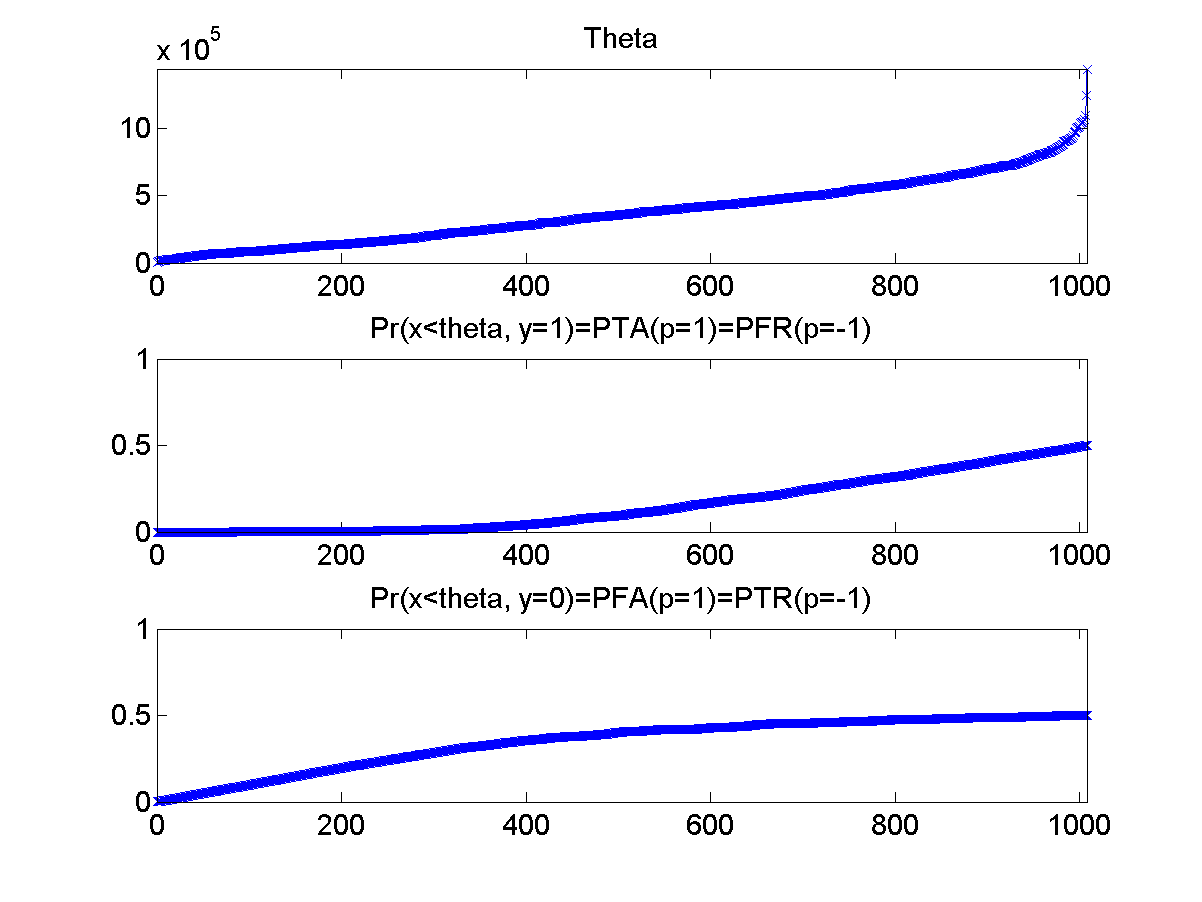
\includegraphics[width=\textwidth]{figs/threshold_falsealarm_falsereject.png}}
    \end{column}
  \end{columns}
\end{frame}

\begin{frame}
  \frametitle{Training Error}

  The probability of error is the probability of false accept, plus
  the probability of false reject.
  If $p_j=+1$:
  \begin{align*}
    \Pr(\text{Error}|p_j=+1)
    &= \Pr(FA|p_j=1) + \Pr(FR|p_j=1)\\
    &= \Pr(FA|p_j=1) + \left(\Pr(y_i=1)-\Pr(TA|p_j=+1)\right)\\
    &=\sum_{i:f_j(x_i)<\theta_j} w_j(x_i)(1-y_i)+P_1-\sum_{i:f_j(x_i)<\theta_j} w_j(x_i)y_i\\
    &=P_1-\sum_{i:f_j(x_i)<\theta_j} w_j(x_i)(2y_i-1),
  \end{align*}
  where $P_1\equiv\Pr(y_i=1)$.  Similarly, if $p_j=-1$:
  \begin{align*}
    \Pr(\text{Error}|p_j=-1)
    &=P_0+\sum_{i:f_j(x_i)<\theta_j} w_j(x_i)(2y_i-1)
  \end{align*}
\end{frame}

\begin{frame}
  \frametitle{Minimum Training Error}
  \begin{align*}
    \Pr(\text{Error}|p_j=1,\theta_j) &=P_1-\sum_{i:f_j(x_i)<\theta_j} w_j(x_i)(2y_i-1)\\
    \Pr(\text{Error}|p_j=-1,\theta_j) &=P_0+\sum_{i:f_j(x_i)<\theta_j} w_j(x_i)(2y_i-1)
  \end{align*}
  \centerline{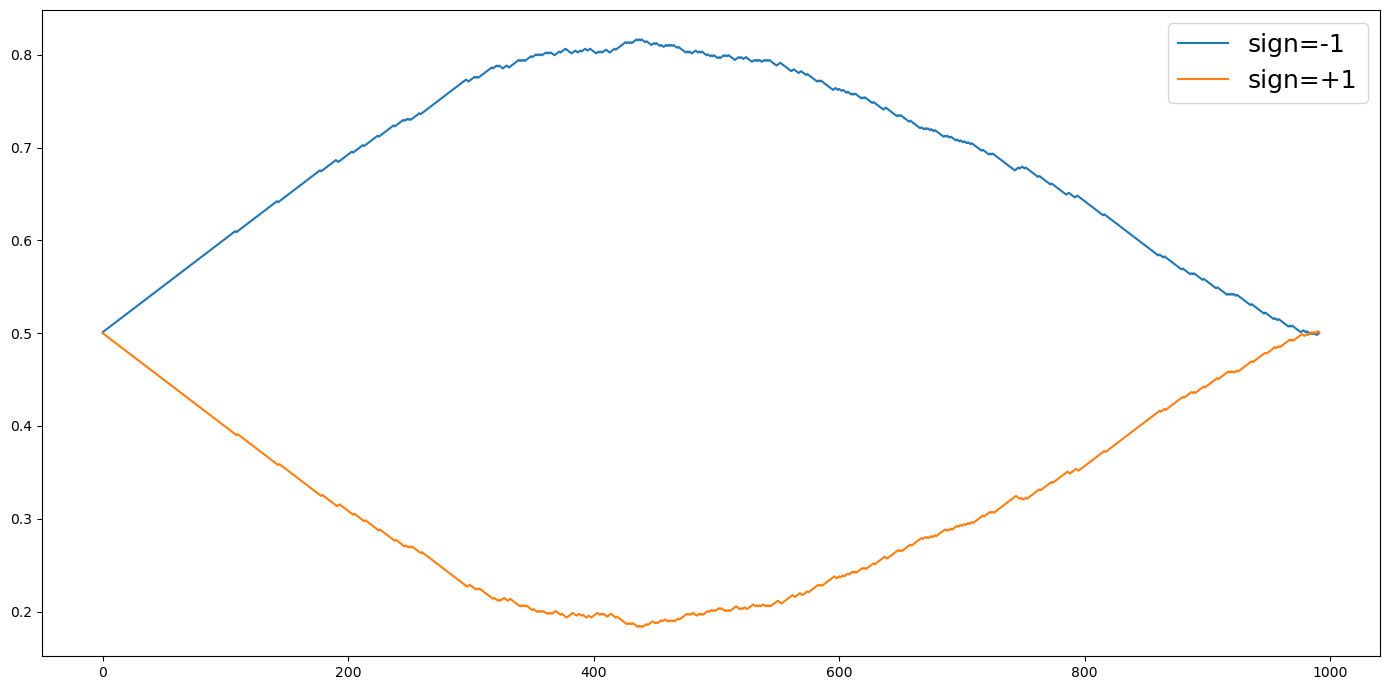
\includegraphics[height=0.5\textheight]{figs/errorplus_errorminus.png}}
\end{frame}

\begin{frame}
  \frametitle{Optimizing the Weak Classifier}

  So, given a particular feature
  $f_j=(\phi_{j,1},\phi_{j,2},\phi_{j,3},\phi_{j,4},o_{j,1},o_{j,2})$,
  we can find the best weak classifier by calculating these two
  curves, and then choosing the value of $p_j$ and $\theta_j$ that
  minimizes the error rate:
  \begin{align*}
    \Pr(\text{Error}|p_j=1,\theta_j) &= P_1-\sum_{i:f_j(x_i)<\theta_j} w_j(x_i)(2y_i-1)\\
    \Pr(\text{Error}|p_j=-1,\theta_j) &= P_0+\sum_{i:f_j(x_i)<\theta_j} w_j(x_i)(2y_i-1)
  \end{align*}
\end{frame}

%%%%%%%%%%%%%%%%%%%%%%%%%%%%%%%%%%%%%%%%%%%%
\section[AdaBoost]{AdaBoost}
\setcounter{subsection}{1}

\begin{frame}
  \frametitle{AdaBoost}

  \begin{itemize}
    \item 
      The AdaBoost algorithm (``adaptive boosting'') is an algorithm that
      combines several weak classifiers in order to form a strong
      classifier.
    \item Suppose that $h_t(x)\in\{0,1\}$ is the $t^{\text{th}}$
      weak classifier
    \item Suppose that $\alpha_t$ is the confidence of the $t^{\text{th}}$ weak classifier
    \item Then the strong classifier's decision is given by:
      \begin{displaymath}
        h(x)=\begin{cases}
        1 & \sum_t \alpha_th_t(x)>\frac{1}{2}\sum_t\alpha_t\\
        0 & \mbox{otherwise}
        \end{cases}
      \end{displaymath}
  \end{itemize}
\end{frame}
    
\begin{frame}
  \frametitle{AdaBoost}

  \begin{displaymath}
    h(x)=\begin{cases}
    1 & \sum_t \alpha_th_t(x)>\frac{1}{2}\sum_t\alpha_t\\
    0 & \mbox{otherwise}
    \end{cases}
  \end{displaymath}

  \begin{itemize}
  \item 
    Notice that this is a kind of neural net.  The first-layer
    excitation is $p_t\theta_t-p_tf_t(x)$, the first-layer
    nonlinearity is a unit step, and the second-layer weights are
    $\alpha_t$.
  \item
    It's like a neural net during training time, but the training
    algorithm is different.
  \end{itemize}
\end{frame}

\begin{frame}
  \frametitle{The AdaBoost Training Algorithm}

  The AdaBoost training algorithm is as follows:
  \begin{enumerate}
  \item {\bf Initialize:} Assign all training tokens the same weight.
  \item {\bf Iterate:} for $t=1,2,\ldots$:
    \begin{enumerate}
    \item Exhaustively test every feature $f_j$:
      \begin{itemize}
      \item Find $p_j$, and $\theta_j$ to minimize the weighted
        training corpus error.
      \end{itemize}
    \item Set $h_t$ equal to the $h_j$ that had the lowest error.
    \item Decrease the weight of the correctly classified tokens, and
      increase the weight of the incorrectly classified tokens.
    \end{enumerate}
  \end{enumerate}
  The result is that each new classifier, $h_t$, is encouraged to try
  to fix the mistakes of all the classifiers that came before it.
\end{frame}

\begin{frame}
  \frametitle{The AdaBoost Training Algorithm}
  \begin{enumerate}
  \item {\bf Initialize:} $w_1(x_i)=1,~~1\le i\le n$.
  \item {\bf Iterate:} for $t=1,2,\ldots$
    \begin{enumerate}
    \item Rescale the weights so they sum to one
    \item Exhaustively test every possible feature.  Find $f_t$,
      $p_t$, and $\theta_t$ to minimize
      \begin{displaymath}
        \epsilon_t = \sum_i w_t(x_i)\vert y_i-h_t(x_i)\vert
      \end{displaymath}
    \item If any training token was correctly classified, decrease its weight by
      \begin{displaymath}
        w_{t+1}(x_i) = \beta_tw_t(x_i),~~~\beta_t =\frac{\epsilon_t}{1-\epsilon_t}
      \end{displaymath}
    \end{enumerate}
  \end{enumerate}
\end{frame}

\begin{frame}[fragile]
  \frametitle{The AdaBoost Training Algorithm}

\begin{lstlisting}
for t in range(T):
  w = w / np.sum(w)
  for theta1 in [0,1/6,2/6,3/6,4/6,5/6]:
    ...
      for theta3 in [1/6,2/6,...,1-theta1]:
        ...
          for o2 in [1,...,4-o1]:
            epsilon = error(theta1,...)
            if epsilon < epsilon_best[t]:
              f[t] = (theta1, theta2, ..., o2)
  beta[t] = epsilon_best[t] / (1-epsilon_best[t])
  w[h == y] *= beta[t]
\end{lstlisting}

\end{frame}


\begin{frame}
  \frametitle{The AdaBoost Training Algorithm}

  Thus, for example, after the first iteration, the weights $w_2(x)$
  have two different magnitudes: those that were correctly classified
  by $h_1(x)$, and those that were incorrectly classified:
  \centerline{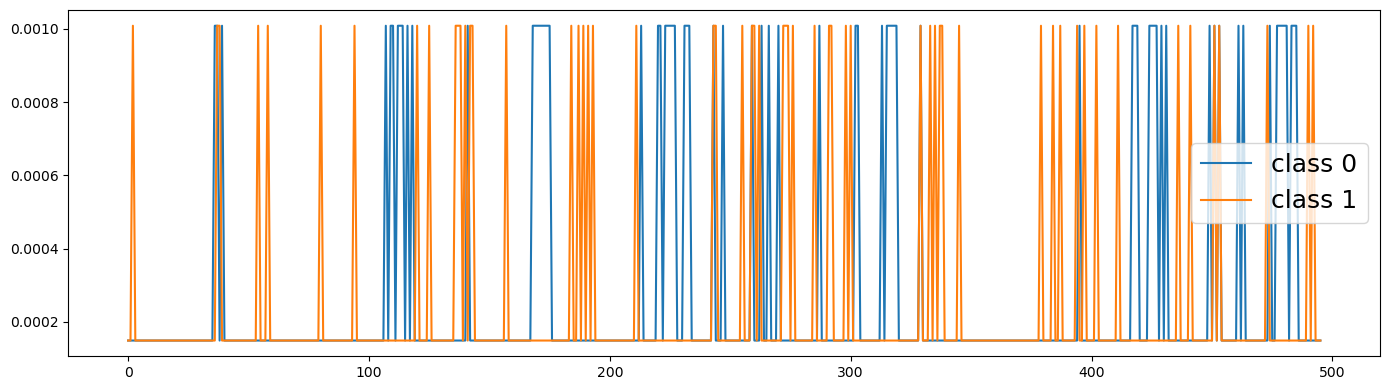
\includegraphics[width=\textwidth]{figs/weights_after_1_iteration.png}}
\end{frame}

\begin{frame}
  \frametitle{The AdaBoost Training Algorithm}
  
  \begin{itemize}
  \item The weighted error rate tends to be lowest in the first
    iteration, and get worse as $t$ gets larger:
    
    \centerline{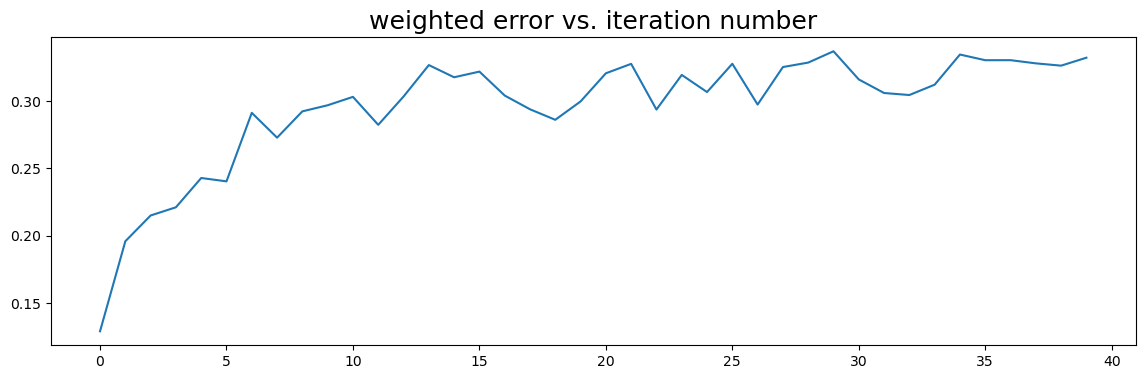
\includegraphics[width=\textwidth]{figs/weightederror_vs_iterationnumber.png}}
  \item That's because, as $t$ increases, the tokens that are hard to
    classify get higher and higher weights, while the easy tokens
    count for less and less.
  \end{itemize}
\end{frame}

\begin{frame}
  \frametitle{AdaBoost Testing}
  \begin{columns}
    \begin{column}{0.5\textwidth}
      In order to test the trained AdaBoost classifier, we use:
      \begin{displaymath}
        h(x)=\begin{cases}
        1 & \sum_t \alpha_th_t(x)>\frac{1}{2}\sum_t\alpha_t\\
        0 & \mbox{otherwise}
        \end{cases},
      \end{displaymath}
      where $\alpha_t=-\ln\beta_t$.
    \end{column}
    \begin{column}{0.5\textwidth}
      Cyan = correct, Magenta = incorrect, Yellow = detected
      \centerline{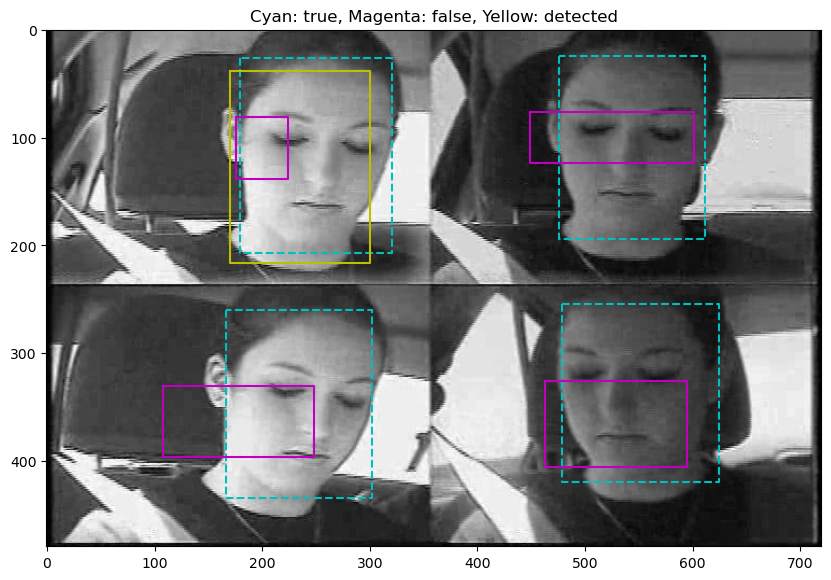
\includegraphics[height=0.7\textheight]{figs/detection_result.png}}
    \end{column}
  \end{columns}
\end{frame}

  
%%%%%%%%%%%%%%%%%%%%%%%%%%%%%%%%%%%%%%%%%%%%
\section[Summary]{Summary}
\setcounter{subsection}{1}

\begin{frame}
  \frametitle{Haar-like Features: Convolutions with Super-low Computation because of the Integral Image}

  \begin{displaymath}
    II[m,n] = \sum_{m'=1}^m\sum_{n'=1^n} I[m',n'],~~~1\le m\le M,1\le n\le N
  \end{displaymath}
  \begin{displaymath}
    \sum_{m'=m}^{m+h}\sum_{n'=n}^{n+w}I[m',n'] = II[m+h,n+w]-II[m,n+w]-II[m+h,n]+II[m,n]
  \end{displaymath}
\end{frame}

\begin{frame}
  \frametitle{The Weak Classifier: Sort the Training Corpus by Feature Value, Choose the Threshold with Lowest Error}

  \begin{align*}
    P_1-\Pr(\text{Error}|p_j=1,\theta_j) &=\\
    \Pr(\text{Error}|p_j=-1,\theta_j)-P_0 &=
    \sum_{i:f_j(x_i)<\theta_j} w_j(x_i)(2y_i-1)
  \end{align*}
\end{frame}

\begin{frame}
  \frametitle{AdaBoost: Each Weak Classifier Tries to Correct the Mistakes of the Ones that Came Before}

  for $t=1,2,\ldots$
  \begin{enumerate}
  \item Rescale the weights so they sum to one
  \item Find $f_t$, $p_t$, and $\theta_t$ to minimize
    \begin{displaymath}
      \epsilon_t = \sum_i w_t(x_i)\vert y_i-h_t(x_i)\vert
    \end{displaymath}
  \item If any training token was correctly classified, decrease its weight by
    \begin{displaymath}
      w_{t+1}(x_i) = \beta_tw_t(x_i),~~~\beta_t =\frac{\epsilon_t}{1-\epsilon_t}
    \end{displaymath}
  \end{enumerate}
  The strong classifier is
  \begin{displaymath}
    h(x)=\begin{cases}
    1 & \sum_t \alpha_th_t(x)>\frac{1}{2}\sum_t\alpha_t\\
    0 & \mbox{otherwise}
    \end{cases},~~~~\alpha_t=-\ln\beta_t
  \end{displaymath}
\end{frame}

\end{document}

